\documentclass[12pt,letterpaper]{article}
\usepackage[utf8]{inputenc}
\usepackage{amsmath}
\usepackage{amsfonts}
\usepackage{amssymb}
\usepackage{float}
\usepackage[margin=0.75in]{geometry}
\usepackage[parfill]{parskip}
\usepackage{graphicx}
\graphicspath{ {images/} }

\usepackage{fancyhdr}
 
\pagestyle{fancy}
\fancyhf{}
\lhead{Andrew Wintenberg}
\rhead{{Page \thepage}}

\linespread{1}

\author{Andrew Wintenberg}
\title{HW2}
\begin{document}

\begin{center}
{\Large \textbf{Homework 2 : ECE 472 }}

{\large Andrew Wintenberg}

{\today}
\end{center}

\thispagestyle{empty}

\section{Introduction}

The objective of this homework was to implement spatial image operations and analyze their effects on image features. Specifically, the operations performed were 3x3 image kernel operations and a 3x3 median filter. Using the provided image of a woman's face (pictured below), the appearance of the resulting images were compared to describe the effect of the operations. In addition, the effects of the complexity of images calculations on computation speed was analyzed by implementing two methods for determining the magnitude of the gradient of an image. One method use the sum of the absolute value of the components and the other used the standard calculation with the square root operation.

All computations were performed using a personal C library written for this course. All images were represented with 8-bit grayscale pixels and stored in the BMP file format.

\begin{figure}[ht]
\centering
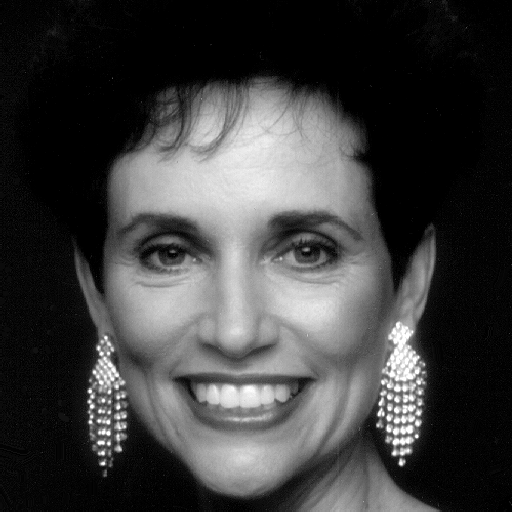
\includegraphics[scale=1.75]{woman/woman} \hspace{0.5cm}
\caption{\small{The original image and on which operations were performed}
\label{fig:base} }
\end{figure}

\newpage

\section{Results}

\subsection{Image Kernels}
Each of the provided image kernel operations were first represented as 3x3 matrix that was then convolved with the provided base image. Note the operation is not well-defined for the pixels on the border as they may not have a full 3x3 neighborhood. In this case, a neighborhood was created by padding the image with zero intensity pixels. The result of each kernel, numbered 1 to 7, is pictured below with the matrix representing the operation and a qualitative description of the result. Note that scaling was performed after each operation to ensure the image was in the range of 0 to 255.

\subsubsection{Image Kernel 1}

The first image kernel averages the pixels in the 3x3 neighborhood of each pixel with equal weight. This results in blurring or smoothing the image which is apparent in the reduction in fine details and the slight reduction in noise in the background.
\begin{figure}[ht]
\centering
$K_1 = \frac{1}{9} \begin{bmatrix}
1 & 1 & 1\\
1 & 1 & 1\\
1 & 1 & 1
\end{bmatrix}$
\hspace{2cm} 
\raisebox{-0.5 \height}{
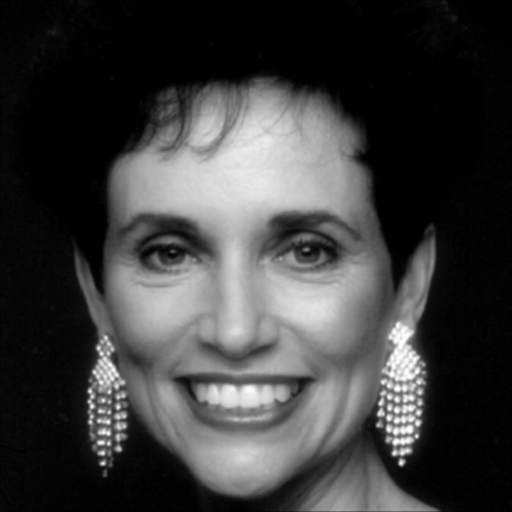
\includegraphics[scale=0.135]{woman/ker1}} 
\caption{\small{The matrix representing the first image kernel and the image after its application}
\label{fig:ker1} }
\end{figure}

\clearpage
\newpage

\subsubsection{Image Kernel 2}

The second image kernel averages the pixels in the 3x3 neighborhood of each pixel. More weight is given to the pixels nearer the original pixel. This results in blurring or smoothing the image which is apparent in the reduction in fine details and the slight reduction in noise in the background. This differs from the first kernel in preserving more of the original image sharpness.
\begin{figure}[ht]
\centering
$K_2 = \frac{1}{16} \begin{bmatrix}
1 & 2 & 1\\
2 & 4 & 2\\
1 & 2 & 1
\end{bmatrix}$
\hspace{2cm} 
\raisebox{-0.5 \height}{
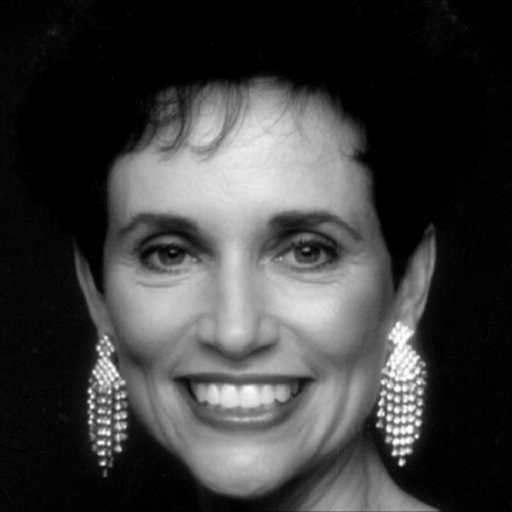
\includegraphics[scale=0.135]{woman/ker2}} 
\caption{\small{The matrix representing the second image kernel and the image after its application}
\label{fig:ker2} }
\end{figure}

\subsubsection{Image Kernel 3}

The third image kernel computes the Laplacian of the image using the adjacent pixels. This is related to the second difference of the image and highlights the edges of the image. This calculation can only capture horizontal and vertical edges.
\begin{figure}[ht]
\centering
$K_3 = \begin{bmatrix}
0 & 1 & 0\\
1 & -4 & 1\\
0 & 1 & 0
\end{bmatrix}$
\hspace{2cm} 
\raisebox{-0.5 \height}{
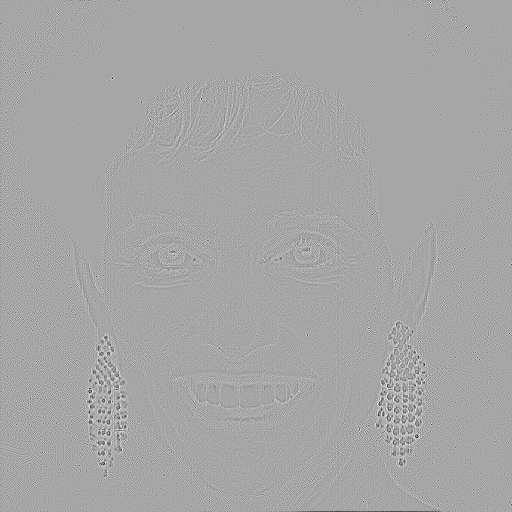
\includegraphics[scale=0.135]{woman/ker3}} 
\caption{\small{The matrix representing the third image kernel and the image after its application}
\label{fig:ker3} }
\end{figure}

\clearpage 
\newpage


\subsubsection{Image Kernel 4}

The fourth image kernel also computes the Laplacian of the image using the pixels in a 3x3 neighborhood. This is related to the second difference of the image and highlights the edges of the image. Unlike the third image kernel, this calculation can capture diagonal edges. Also note that the noise in the image such as in the background and the face is emphasized.
\begin{figure}[ht]
\centering
$K_4 =  \begin{bmatrix}
1 & 1 & 1\\
1 & -8 & 1\\
1 & 1 & 1
\end{bmatrix}$
\hspace{2cm} 
\raisebox{-0.5 \height}{
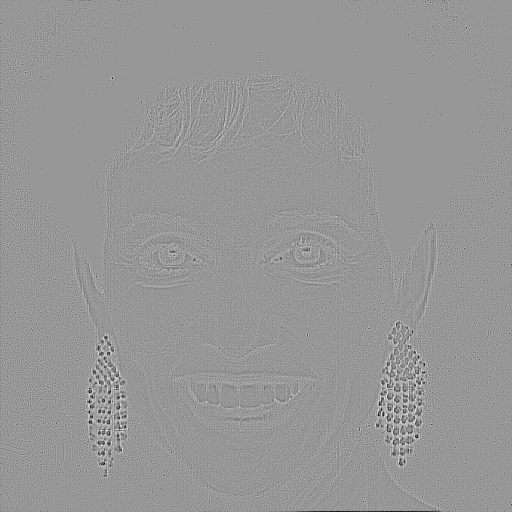
\includegraphics[scale=0.135]{woman/ker4}} 
\caption{\small{The matrix representing the third image kernel and the image after its application}
\label{fig:ker4} }
\end{figure}

\subsubsection{Image Kernel 5}

The fifth image kernel also computes the inverse or negative of the Laplacian of the image using the adjacent pixels. The result is the negative or the result of the fourth kernel. This sharpens the image.
\begin{figure}[ht]
\centering
$K_5 = \begin{bmatrix}
0 & -1 & 0\\
-1 & 4 & -1\\
0 & -1 & 0
\end{bmatrix}$
\hspace{2cm} 
\raisebox{-0.5 \height}{
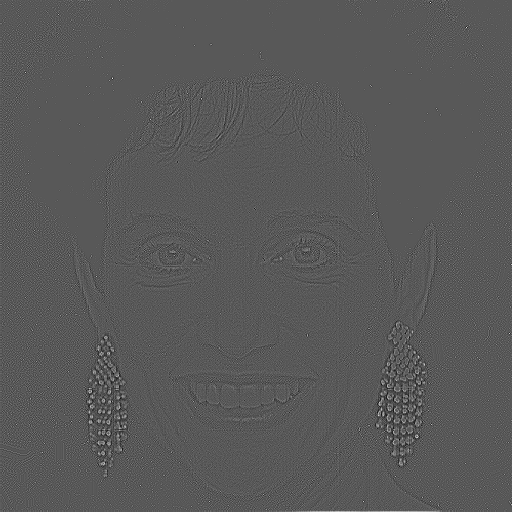
\includegraphics[scale=0.135]{woman/ker5}} 
\caption{\small{The matrix representing the fifth image kernel and the image after its application}
\label{fig:ker5} }
\end{figure}

\clearpage 
\newpage

\subsubsection{Image Kernel 6}

The sixth image kernel also computes the derivative in the vertical direction of the image using the pixels in a 3x3 neighborhood. This greatly emphasizes the horizontal edges of the image.
\begin{figure}[ht]
\centering
$K_5 = \begin{bmatrix}
-1 & -2 & -1\\
0 & 0 & 0\\
1 & 2 & 1
\end{bmatrix}$
\hspace{2cm} 
\raisebox{-0.5 \height}{
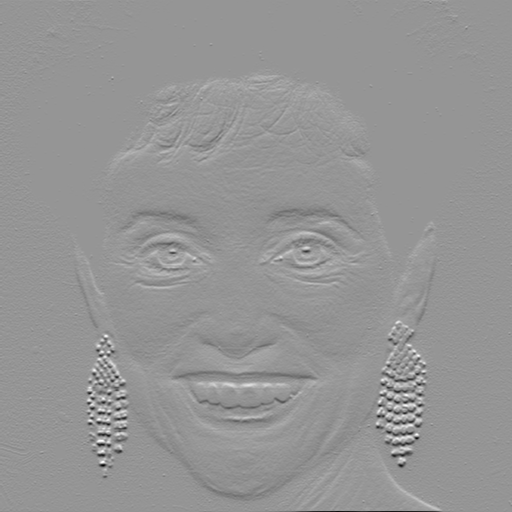
\includegraphics[scale=0.135]{woman/ker6}} 
\caption{\small{The matrix representing the sixth image kernel and the image after its application}
\label{fig:ker6} }
\end{figure}

\subsubsection{Image Kernel 7}

The seventh image kernel also computes the derivative but in the horizontal direction using the pixels in a 3x3 neighborhood. This greatly emphasizes the vertical edges of the image.
\begin{figure}[ht]
\centering
$K_5 = \begin{bmatrix}
-1 & 0 & 1\\
-2 & 0 & 2\\
-1 & 0 & 1
\end{bmatrix}$
\hspace{2cm} 
\raisebox{-0.5 \height}{
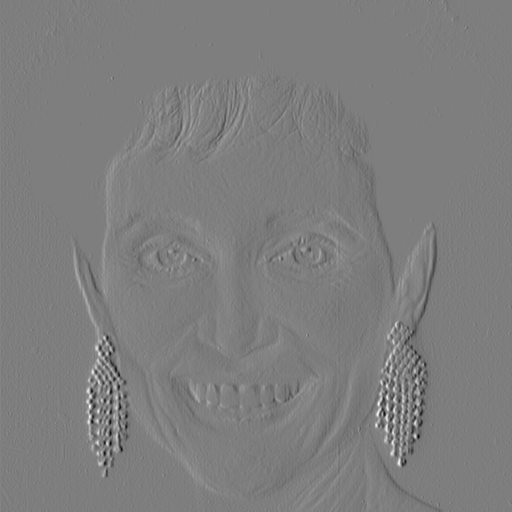
\includegraphics[scale=0.135]{woman/ker7}} 
\caption{\small{The matrix representing the seventh image kernel and the image after its application}
\label{fig:ker7} }
\end{figure}

\clearpage 
\newpage

\section{Varying Image Kernel}
In this section, the following kernel is applied with varying values of $A$ \[
K_{8,A}\begin{bmatrix}
-1 & -1 & -1 \\
-1 & 8 + A & -1\\
-1 & -1 & -1 \\
\end{bmatrix}
\]
As $A$ is decreased, the resulting images transition from the original to a sharpened version. The values of $A$ used were $0, 1, 2, 4, 8$ and the results are pictured below.

\begin{figure}[ht]
\centering
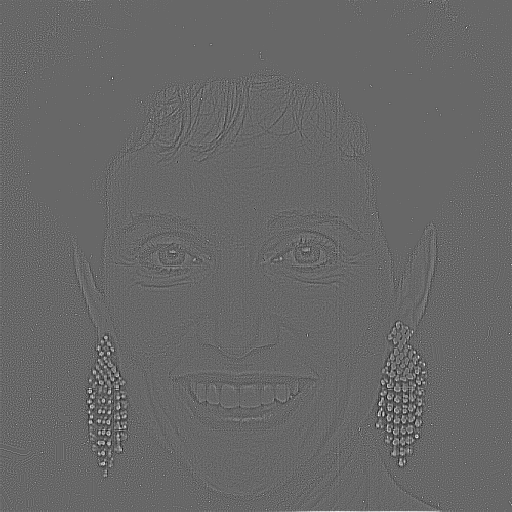
\includegraphics[scale=0.135]{woman/ker_a0}
\caption{\small{The image resulting from setting A = 0}
\label{fig:ker_a0} }
\end{figure}
\begin{figure}[ht]
\centering
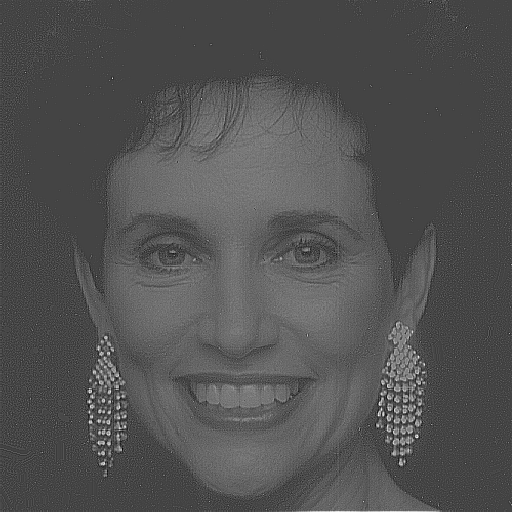
\includegraphics[scale=0.135]{woman/ker_a1}
\caption{\small{The image resulting from setting A = 1}
\label{fig:ker_a1} }
\end{figure}

\clearpage 
\newpage

\begin{figure}[ht]
\centering
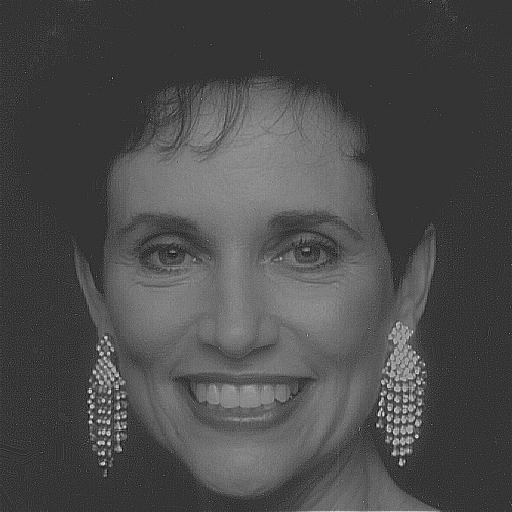
\includegraphics[scale=0.135]{woman/ker_a2}
\caption{\small{The image resulting from setting A = 2}
\label{fig:ker_a2} }
\end{figure}
\begin{figure}[ht]
\centering
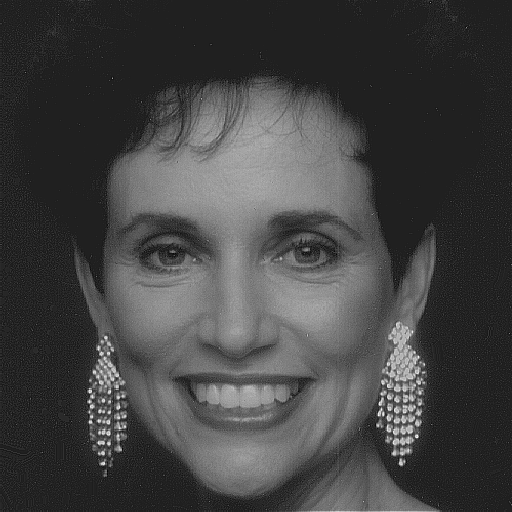
\includegraphics[scale=0.135]{woman/ker_a4}
\caption{\small{The image resulting from setting A = 4}
\label{fig:ker_a4} }
\end{figure}
\clearpage 
\newpage

\begin{figure}[ht]
\centering
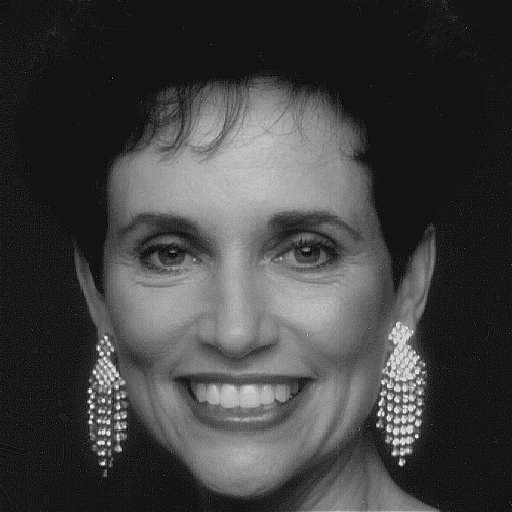
\includegraphics[scale=0.135]{woman/ker_a8}
\caption{\small{The image resulting from setting A = 8}
\label{fig:ker_a8} }
\end{figure}

\begin{figure}[ht]
\centering
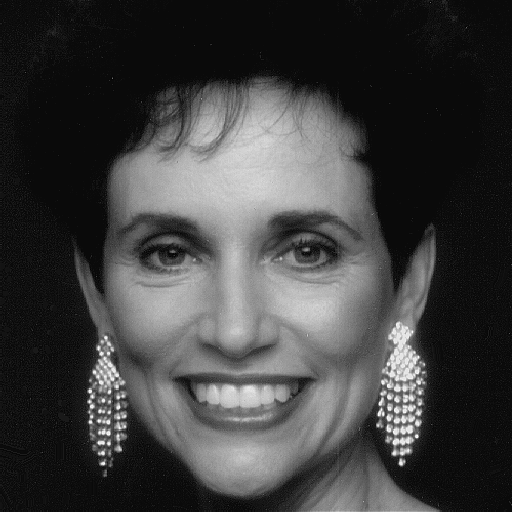
\includegraphics[scale=0.135]{woman/ker_a16}
\caption{\small{The image resulting from setting A = 16}
\label{fig:ker_a16} }
\end{figure}

\clearpage 
\newpage

\section{Median Filter}

In this section a median filter was applied to the base image. The filtered pixel intensity is equal to the median intensity of the original pixel's 3x3 neighborhood, padded with zero as necessary. This filter smooths the image and can remove certain types of noise such as "salt and pepper noise". 

\begin{figure}[ht]
\centering
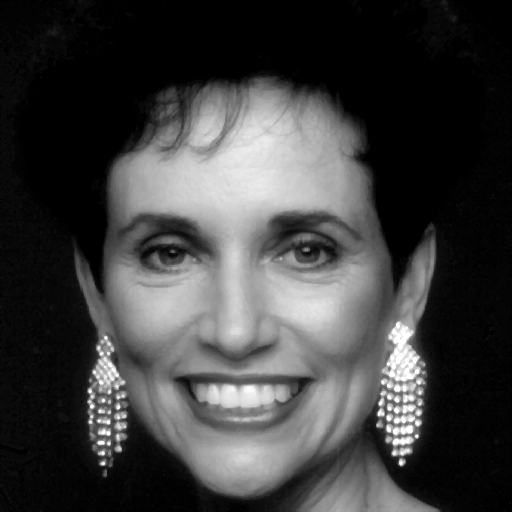
\includegraphics[scale=0.135]{woman/median} 
\caption{\small{The image after application of the median filter}
\label{fig:med} }
\end{figure}

\clearpage 
\newpage
\section{Gradient Computation Speed}
In this section the magnitude of the gradient of the image was computed using the exact method \[
||\nabla f|| = \sqrt{ \left( \frac{\partial}{\partial x} f \right)^2 + \left( \frac{\partial}{\partial y} f \right)^2} = \frac{1}{4} \sqrt{(f(i + 1, j) - f(i - 1, j))^2 + (f(i, j + 1) - f(i, j - 1))^2}
\]
and an approximate method using the absolute value \[
||\nabla f|| = \left|\frac{\partial}{\partial x} f\right| + \left| \frac{\partial}{\partial y} f \right| = \frac{1}{2}\left(|f(i + 1, j) - f(i - 1, j)| + |f(i, j + 1) - f(i, j - 1)|\right)
\]

For each method the gradient was computed 100 times on the base image (512x512) to find the average computation time. In particular the standard $sqrt$ and $fabs$   The results are as follows \[
T_{exact} = 0.09713s \qquad \qquad T_{approx} = 0.0164s
\]
As expected the approximation computation  was much quicker than the exact computation. Note that a non-trivial amount of computation time is spent on memory manipulation.


\section{Conclusion}
In conclusion, the various spatial operations performed on an image can emphasize certain image features such as as edges. In addition, due to the computationally intensive nature of image processing, approximations can be valuable to reduce computation time.

\end{document}